\documentclass[11pt,a4paper]{report}
\usepackage[textwidth=37em,vmargin=30mm]{geometry}
\usepackage{calc,xunicode,amsmath,amssymb,paralist,enumitem,tabu,booktabs,datetime2,xeCJK,xeCJKfntef,listings}
\usepackage{tocloft,fancyhdr,tcolorbox,xcolor,graphicx,eso-pic,xltxtra,xelatexemoji}

\newcommand{\envyear}[0]{2025}
\newcommand{\envdatestr}[0]{2025-08-09}
\newcommand{\envfinaldir}[0]{webdb/2025/20250809/final}

\usepackage[hidelinks]{hyperref}
\hypersetup{
    colorlinks=false,
    pdfpagemode=FullScreen,
    pdftitle={Web Digest - \envdatestr}
}

\setlength{\cftbeforechapskip}{10pt}
\renewcommand{\cftchapfont}{\rmfamily\bfseries\large\raggedright}
\setlength{\cftbeforesecskip}{2pt}
\renewcommand{\cftsecfont}{\sffamily\small\raggedright}

\setdefaultleftmargin{2em}{2em}{1em}{1em}{1em}{1em}

\usepackage{xeCJK,xeCJKfntef}
\xeCJKsetup{PunctStyle=plain,RubberPunctSkip=false,CJKglue=\strut\hskip 0pt plus 0.1em minus 0.05em,CJKecglue=\strut\hskip 0.22em plus 0.2em}
\XeTeXlinebreaklocale "zh"
\XeTeXlinebreakskip = 0pt


\setmainfont{Brygada 1918}
\setromanfont{Brygada 1918}
\setsansfont{IBM Plex Sans}
\setmonofont{JetBrains Mono NL}
\setCJKmainfont{Noto Serif CJK SC}
\setCJKromanfont{Noto Serif CJK SC}
\setCJKsansfont{Noto Sans CJK SC}
\setCJKmonofont{Noto Sans CJK SC}

\setlength{\parindent}{0pt}
\setlength{\parskip}{8pt}
\linespread{1.15}

\lstset{
	basicstyle=\ttfamily\footnotesize,
	numbersep=5pt,
	backgroundcolor=\color{black!5},
	showspaces=false,
	showstringspaces=false,
	showtabs=false,
	tabsize=2,
	captionpos=b,
	breaklines=true,
	breakatwhitespace=true,
	breakautoindent=true,
	linewidth=\textwidth
}






\newcommand{\coverpic}[2]{
    % argv: itemurl, authorname
    Cover photo by #2~~(\href{#1}{#1})
}
\newcommand{\makeheader}[0]{
    \begin{titlepage}
        % \newgeometry{hmargin=15mm,tmargin=21mm,bmargin=12mm}
        \begin{center}
            
            \rmfamily\scshape
            \fontspec{BaskervilleF}
            \fontspec{Old Standard}
            \fontsize{59pt}{70pt}\selectfont
            WEB\hfill DIGEST
            
            \vfill
            % \vskip 30pt
            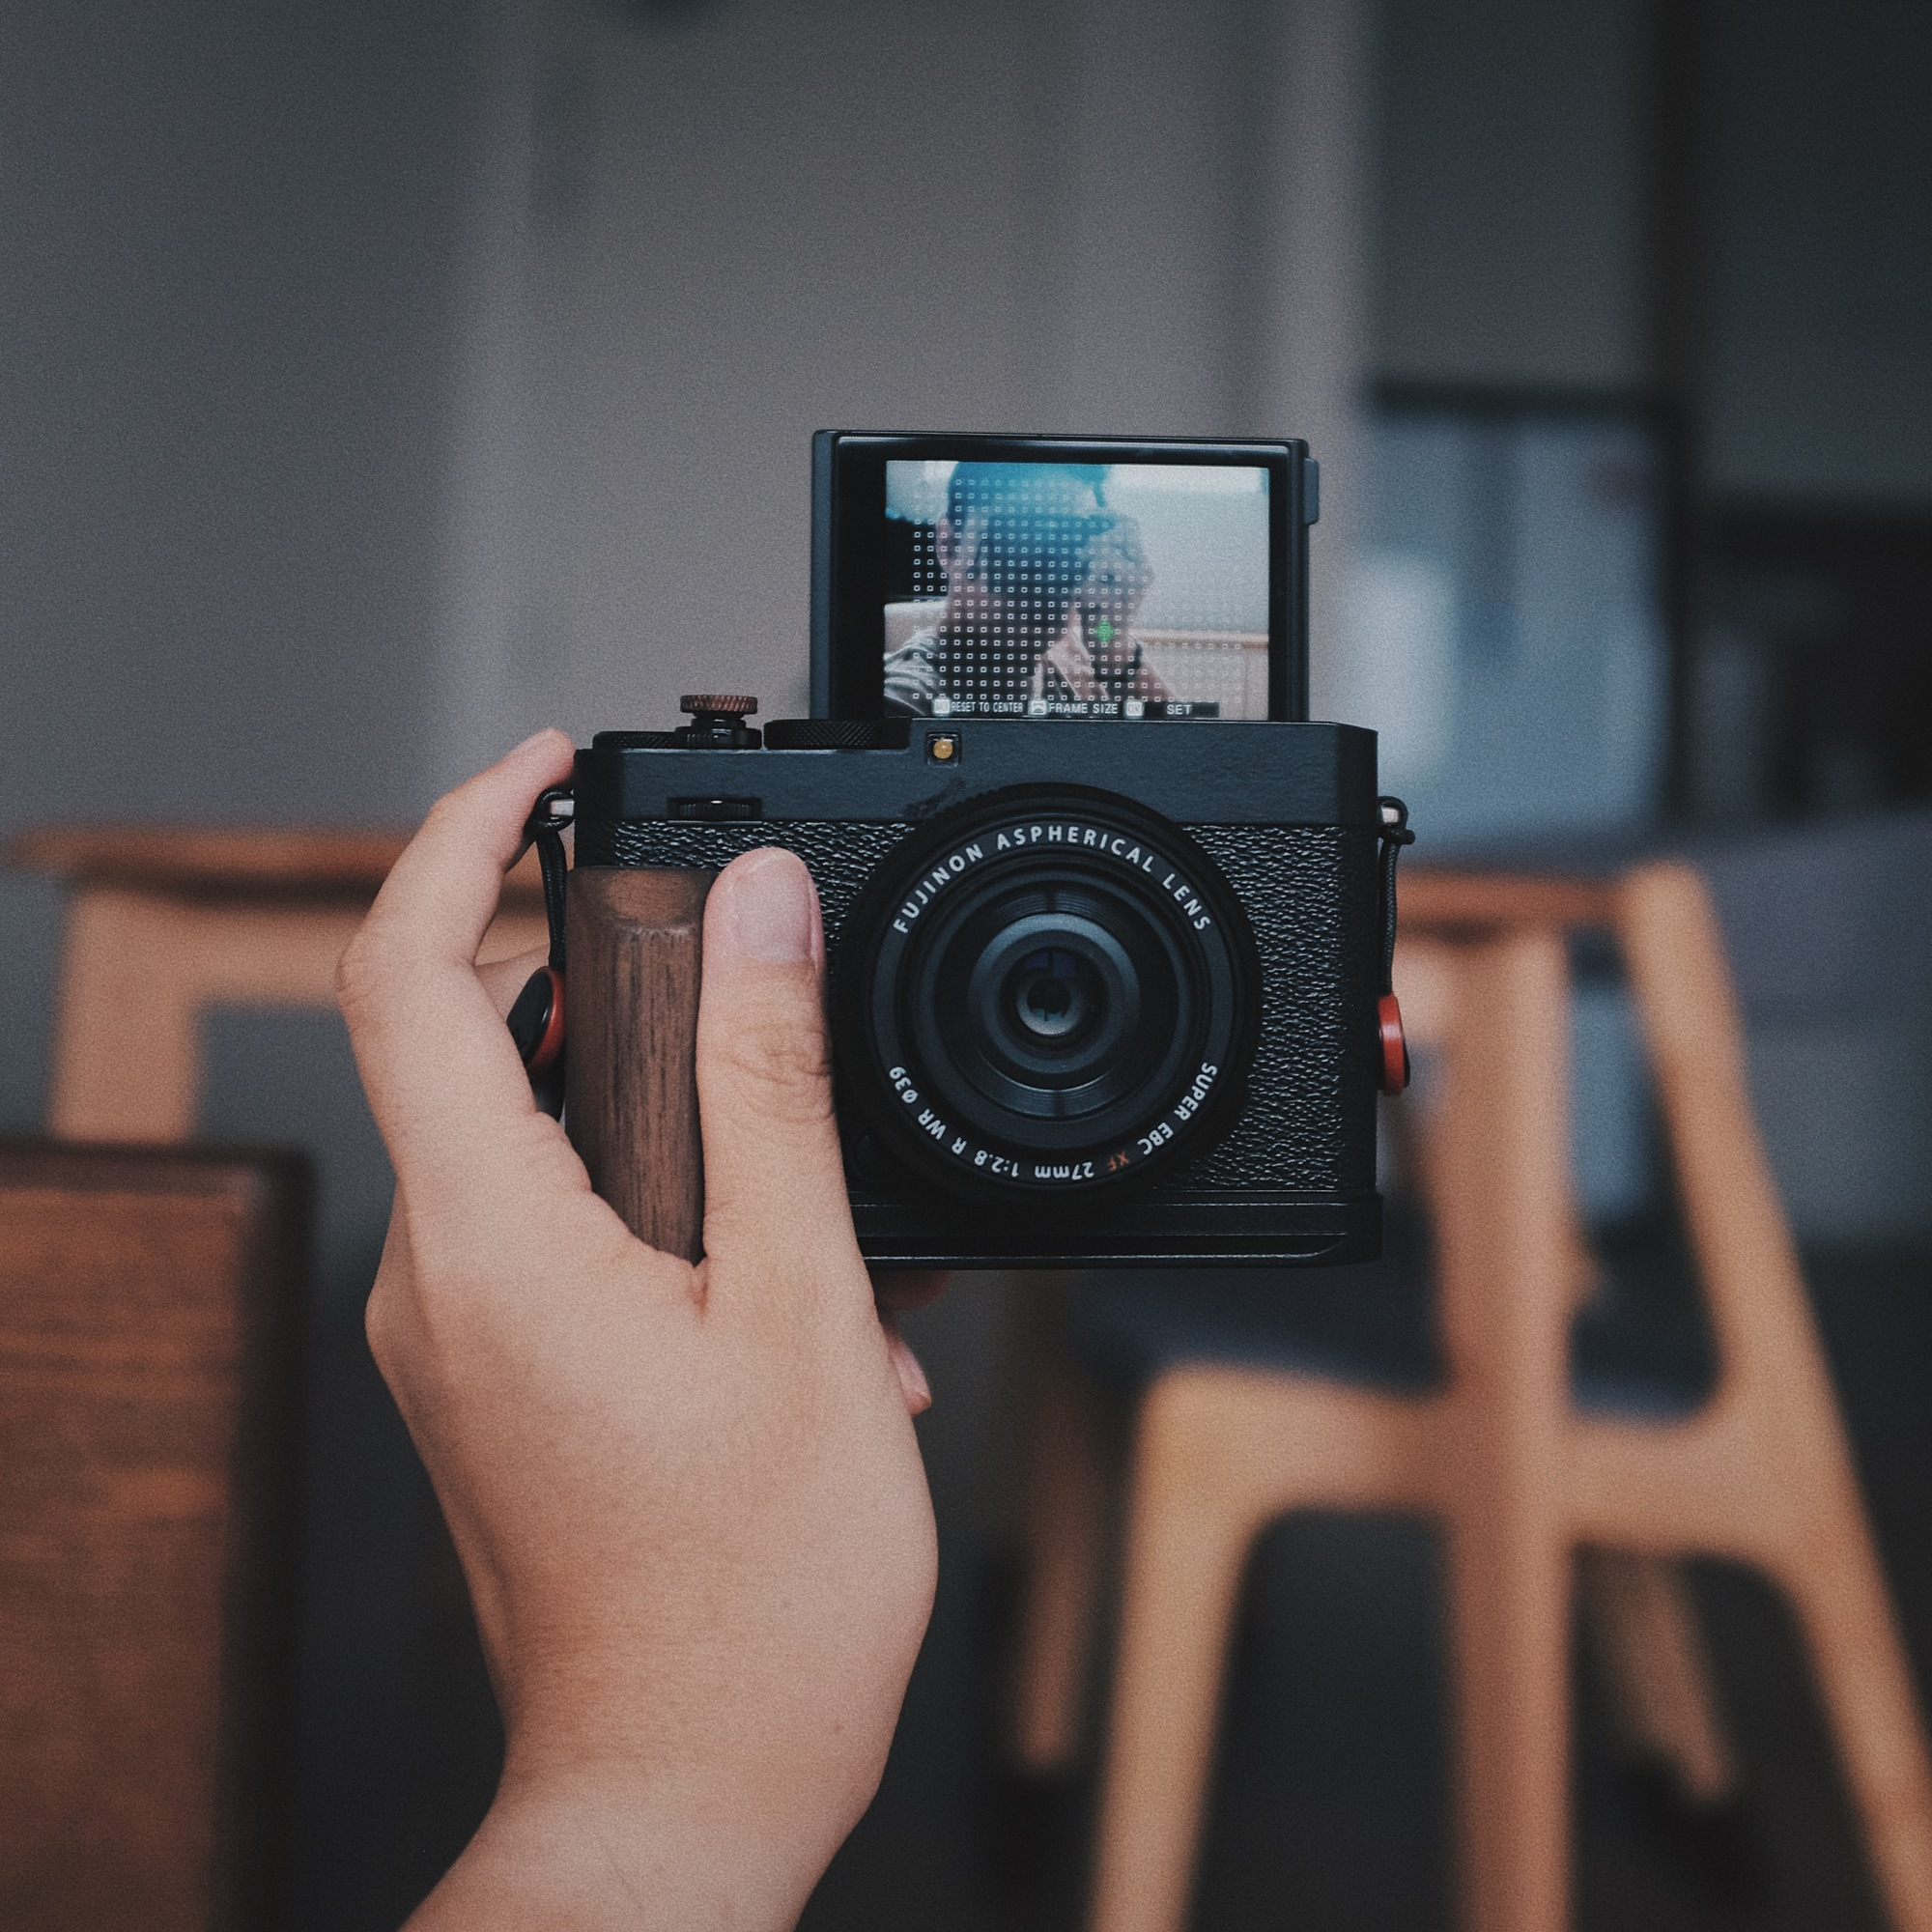
\includegraphics[width=\linewidth]{\envfinaldir/coverpic-prod.jpg}\par
            % \vskip 30pt
            \vfill

            \normalsize\rmfamily\scshape
            \copyright{} The Web Digest Project \hfill\large \envdatestr
        \end{center}
    \end{titlepage}
    % \restoregeometry
}
\newcommand{\simplehref}[1]{%
    \textcolor{blue!80!green}{\href{#1}{#1}}%
}
\renewcommand{\contentsname}{\center\Huge\sffamily\bfseries Contents\par\vskip 20pt}
\newcounter{ipartcounter}
\setcounter{ipartcounter}{0}
\newcommand{\ipart}[1]{
    % \vskip 20pt
    \clearpage
    \stepcounter{ipartcounter}
    \phantomsection
    \addcontentsline{toc}{chapter}{#1}
    % \begin{center}
    %     \Huge
    %     \sffamily\bfseries
    %     #1
    % \end{center}
    % \vskip 20pt plus 7pt
}
\newcounter{ichaptercounter}
\setcounter{ichaptercounter}{0}
\newcommand{\ichapter}[1]{
    % \vskip 20pt
    \clearpage
    \stepcounter{ichaptercounter}
    \phantomsection
    \addcontentsline{toc}{section}{\numberline{\arabic{ichaptercounter}}#1}
    \begin{center}
        \Huge
        \sffamily\bfseries
        #1
    \end{center}
    \vskip 20pt plus 7pt
}
\newcommand{\entrytitlefont}[1]{\subsection*{\raggedright\Large\sffamily\bfseries#1}}
\newcommand{\entryitemGeneric}[2]{
    % argv: title, url
    \parbox{\linewidth}{
        \entrytitlefont{#1}\par\vskip 5pt
        \footnotesize\ttfamily\mdseries
        \simplehref{#2}
    }\vskip 11pt plus 11pt minus 1pt
}
\newcommand{\entryitemGithub}[3]{
    % argv: title, url, desc
    \parbox{\linewidth}{
        \entrytitlefont{#1}\par\vskip 5pt
        \footnotesize\ttfamily\mdseries
        \simplehref{#2}\par\vskip 5pt
        \small\rmfamily\mdseries#3
    }\vskip 11pt plus 11pt minus 1pt
}
\newcommand{\entryitemAp}[3]{
    % argv: title, url, desc
    \parbox{\linewidth}{
        \entrytitlefont{#1}\par\vskip 5pt
        \footnotesize\ttfamily\mdseries
        \simplehref{#2}\par\vskip 5pt
        \small\rmfamily\mdseries#3
    }\vskip 11pt plus 11pt minus 1pt
}
\newcommand{\entryitemHackernews}[3]{
    % argv: title, hnurl, rawurl
    % \parbox{\linewidth}{
    %     \entrytitlefont{#1}\par\vskip 5pt
    %     \footnotesize\ttfamily\mdseries
    %     \simplehref{#3}\par
    %     \textcolor{black!50}{\href{#2}{#2}}
    % }\vskip 11pt plus 11pt minus 1pt
    \begin{minipage}{\linewidth}
            \entrytitlefont{#1}\par\vskip 5pt
            \footnotesize\ttfamily\mdseries
            \simplehref{#3}\par
            \textcolor{black!50}{\href{#2}{#2}}
    \end{minipage}\par\vskip 11pt plus 11pt minus 1pt
}







\begin{document}

\makeheader

\tableofcontents\clearpage




\ipart{Developers}
\ichapter{Hacker News}
\entryitemTwoLinks{Ask HN: How can ChatGPT serve 700M users when I can't run one GPT-4 locally?}{https://news.ycombinator.com/item?id=44840728}{https://news.ycombinator.com/item?id=44840728}

\entryitemTwoLinks{Jim Lovell, Apollo 13 commander, has died}{https://news.ycombinator.com/item?id=44840582}{https://www.nasa.gov/news-release/acting-nasa-administrator-reflects-on-legacy-of-astronaut-jim-lovell/}

\entryitemTwoLinks{I want everything local – Building my offline AI workspace}{https://news.ycombinator.com/item?id=44840013}{https://instavm.io/blog/building-my-offline-ai-workspace}

\entryitemTwoLinks{The surprise deprecation of GPT-4o for ChatGPT consumers}{https://news.ycombinator.com/item?id=44839842}{https://simonwillison.net/2025/Aug/8/surprise-deprecation-of-gpt-4o/}

\entryitemTwoLinks{A message from Intel CEO Lip-Bu Tan to all company employees}{https://news.ycombinator.com/item?id=44839705}{https://newsroom.intel.com/corporate/my-commitment-to-you-and-our-company}

\entryitemTwoLinks{Tor: How a military project became a lifeline for privacy}{https://news.ycombinator.com/item?id=44838378}{https://thereader.mitpress.mit.edu/the-secret-history-of-tor-how-a-military-project-became-a-lifeline-for-privacy/}

\entryitemTwoLinks{GPT-5 vs. Sonnet: Complex Agentic Coding}{https://news.ycombinator.com/item?id=44838303}{https://elite-ai-assisted-coding.dev/p/copilot-agentic-coding-gpt-5-vs-claude-4-sonnet}

\entryitemTwoLinks{AI must RTFM: Why tech writers are becoming context curators}{https://news.ycombinator.com/item?id=44837875}{https://passo.uno/from-tech-writers-to-ai-context-curators/}

\entryitemTwoLinks{AI is impressive because we've failed at personal computing}{https://news.ycombinator.com/item?id=44837783}{https://rakhim.exotext.com/ai-is-impressive-because-we-ve-failed-at-semantic-web-and-personal-computing}

\entryitemTwoLinks{Google's Genie is more impressive than GPT5}{https://news.ycombinator.com/item?id=44837646}{https://theahura.substack.com/p/tech-things-genies-lamp-openai-cant}

\entryitemTwoLinks{Astronomy Photographer of the Year 2025 shortlist}{https://news.ycombinator.com/item?id=44837434}{https://www.rmg.co.uk/whats-on/astronomy-photographer-year/galleries/2025-shortlist}

\entryitemTwoLinks{Getting good results from Claude Code}{https://news.ycombinator.com/item?id=44836879}{https://www.dzombak.com/blog/2025/08/getting-good-results-from-claude-code/}

\entryitemTwoLinks{How we replaced Elasticsearch and MongoDB with Rust and RocksDB}{https://news.ycombinator.com/item?id=44836463}{https://radar.com/blog/high-performance-geocoding-in-rust}

\entryitemTwoLinks{Food, housing, \& health care costs are a source of major stress for many people}{https://news.ycombinator.com/item?id=44836219}{https://apnorc.org/projects/food-housing-and-health-care-costs-are-a-source-of-major-stress-for-many-people/}

\entryitemTwoLinks{Ultrathin business card runs a fluid simulation}{https://news.ycombinator.com/item?id=44835879}{https://github.com/Nicholas-L-Johnson/flip-card}

\entryitemTwoLinks{US to rewrite its past national climate reports}{https://news.ycombinator.com/item?id=44835287}{https://www.france24.com/en/live-news/20250807-us-to-rewrite-its-past-national-climate-reports}

\entryitemTwoLinks{How attention sinks keep language models stable}{https://news.ycombinator.com/item?id=44834918}{https://hanlab.mit.edu/blog/streamingllm}

\entryitemTwoLinks{Linear sent me down a local-first rabbit hole}{https://news.ycombinator.com/item?id=44833834}{https://bytemash.net/posts/i-went-down-the-linear-rabbit-hole/}

\entryitemTwoLinks{GPT-5 leaked system prompt?}{https://news.ycombinator.com/item?id=44832990}{https://gist.github.com/maoxiaoke/f6d5b28f9104cd856a2622a084f46fd7}

\entryitemTwoLinks{New executive order puts all grants under political control}{https://news.ycombinator.com/item?id=44832829}{https://arstechnica.com/science/2025/08/new-executive-order-puts-all-grants-under-political-control/}\ichapter{Phoronix}
\entryitemGeneric{\hskip 0pt{}Additional Intel Linux Drivers Left Orphaned \& Maintainers Let Go}{https://www.phoronix.com/news/Intel-More-Orphans-Maintainers}

\entryitemGeneric{\hskip 0pt{}Intel CPU Temperature Monitoring Driver For Linux Now Unmaintained After Layoffs}{https://www.phoronix.com/news/Linux-coretemp-Orphaned}

\entryitemGeneric{\hskip 0pt{}Bcachefs Maintainer Comments On The LKML While Waiting To See What Happens}{https://www.phoronix.com/news/Bcachefs-Linux-6.18-Waits}

\entryitemGeneric{\hskip 0pt{}AMD Linux Driver Prepares For Radeon RDNA4 "Kicker"}{https://www.phoronix.com/news/AMD-RDNA4-Kicker-Linux}

\entryitemGeneric{\hskip 0pt{}DDR5-6400 vs. DDR5-4800 R-DIMM Performance For Threadripper 9980X / 9970X CPUs}{https://www.phoronix.com/review/threadripper-9000-ddr5-6400-4800}

\entryitemGeneric{\hskip 0pt{}AMD ROCm 6.4.3 Released With A Few Fixes}{https://www.phoronix.com/news/AMD-ROCm-6.4.3}

\entryitemGeneric{\hskip 0pt{}LVFS Introducing Fair-Use Quota: Asking Major Vendors To Pay Or Contribute Code}{https://www.phoronix.com/news/LVFS-Fair-Use-Quota}

\entryitemGeneric{\hskip 0pt{}RADV Implements Triangle Pair Compression For AMD RDNA4 GPUs}{https://www.phoronix.com/news/RADV-RDNA4-Tri-Pair-Compress}

\entryitemGeneric{\hskip 0pt{}PCIe Improvements With Linux 6.17: Intel Panther Lake, Qualcomm, Sophgo SG2044 \& More}{https://www.phoronix.com/news/Linux-6.17-PCI-PCIe}


\ipart{Developers~~~~(zh-Hans)}
\ichapter{Solidot}
\entryitemGeneric{\hskip 0pt{}中国主要太阳能公司去年裁员近三分之一}{https://www.solidot.org/story?sid=81994}

\entryitemGeneric{\hskip 0pt{}Windows 10 的 30 美元扩展安全更新支持单一账号 10 台设备}{https://www.solidot.org/story?sid=81993}

\entryitemGeneric{\hskip 0pt{}Linux 桌面市场份额达到 6\%}{https://www.solidot.org/story?sid=81992}

\entryitemGeneric{\hskip 0pt{}OpenAI 发布 GPT-5}{https://www.solidot.org/story?sid=81991}

\entryitemGeneric{\hskip 0pt{}科学家重新创造宇宙第一种分子}{https://www.solidot.org/story?sid=81990}

\entryitemGeneric{\hskip 0pt{}研究显示大模型生成虚假临床信息的可能性高于五成}{https://www.solidot.org/story?sid=81989}

\entryitemGeneric{\hskip 0pt{}特朗普呼吁陈立武立即辞职}{https://www.solidot.org/story?sid=81988}

\entryitemGeneric{\hskip 0pt{}以色列在微软服务器上储存了数百万巴勒斯坦人的电话呼叫}{https://www.solidot.org/story?sid=81987}

\entryitemGeneric{\hskip 0pt{}来自深海细菌的多糖能导致癌细胞自毁}{https://www.solidot.org/story?sid=81986}

\entryitemGeneric{\hskip 0pt{}日本人口连续 16 年减少}{https://www.solidot.org/story?sid=81985}

\entryitemGeneric{\hskip 0pt{}《战地6》和《使命召唤 黑色行动 7》都要求 PC 玩家启用 Secure Boot}{https://www.solidot.org/story?sid=81984}

\entryitemGeneric{\hskip 0pt{}特朗普威胁对芯片征收 100\% 关税,除非在美建厂或承诺建厂}{https://www.solidot.org/story?sid=81983}

\entryitemGeneric{\hskip 0pt{}日本禁止苹果 iOS 限制第三方浏览器引擎}{https://www.solidot.org/story?sid=81982}

\entryitemGeneric{\hskip 0pt{}Grok 未经用户要求就生成斯威夫特的裸照}{https://www.solidot.org/story?sid=81981}

\entryitemGeneric{\hskip 0pt{}维基百科编辑对 AI 生成文章采用加速删除政策}{https://www.solidot.org/story?sid=81980}

\entryitemGeneric{\hskip 0pt{}GitHub CEO 警告开发者要么拥抱 AI 要么改行}{https://www.solidot.org/story?sid=81979}

\entryitemGeneric{\hskip 0pt{}Proxmox Virtual Environment 9.0 释出}{https://www.solidot.org/story?sid=81978}

\entryitemGeneric{\hskip 0pt{}瑞典首相因在工作中使用 AI 工具而受到批评}{https://www.solidot.org/story?sid=81977}

\entryitemGeneric{\hskip 0pt{}OpenAI 自 GPT-2 以来首次发布开放权重模型}{https://www.solidot.org/story?sid=81976}

\entryitemGeneric{\hskip 0pt{}美科技企业今年前七个月裁员 9 万人}{https://www.solidot.org/story?sid=81975}\ichapter{V2EX}
\entryitemGeneric{\hskip 0pt{}[音乐] Android 电视上有没有什么好用的音乐播放器}{https://www.v2ex.com/t/1151160}

\entryitemGeneric{\hskip 0pt{}[宽带症候群] 临时申请了一部分 9929 体验名额}{https://www.v2ex.com/t/1151159}

\entryitemGeneric{\hskip 0pt{}[Solana] 准备跑步入场,没想到 C2C 买币无法成功}{https://www.v2ex.com/t/1151158}

\entryitemGeneric{\hskip 0pt{}[问与答] TOP 主题各种 \$V2EX ,求一个可以过滤方式}{https://www.v2ex.com/t/1151157}

\entryitemGeneric{\hskip 0pt{}[Solana] Awesome V2EX}{https://www.v2ex.com/t/1151156}

\entryitemGeneric{\hskip 0pt{}[Solana] 为什么有两个地址频繁买卖,但是查不到交易记录,导致\$v2ex 暴跌}{https://www.v2ex.com/t/1151155}

\entryitemGeneric{\hskip 0pt{}[问与答] 我想关闭 windows 更新以及阻止信息的收集,有人推荐 Atlas-OS 这个软件,不知道有没有人用过,使用感受如何?会不会影响日常操作?}{https://www.v2ex.com/t/1151152}

\entryitemGeneric{\hskip 0pt{}[Solana] 我也有币啦😎}{https://www.v2ex.com/t/1151150}

\entryitemGeneric{\hskip 0pt{}[酷工作] 900+ 岗位内推,早 9 晚 6,双休,校招/社招,技术/非技术}{https://www.v2ex.com/t/1151149}

\entryitemGeneric{\hskip 0pt{}[程序员] claude 的 ip 审查网页和 api 是不同的吗?}{https://www.v2ex.com/t/1151148}

\entryitemGeneric{\hskip 0pt{}[Solana] 为什么无法购买 \$V2EX}{https://www.v2ex.com/t/1151146}

\entryitemGeneric{\hskip 0pt{}[程序员] 关于沉浸式翻译计划禁用一些第三方自定义 key 提供方的补充说明}{https://www.v2ex.com/t/1151145}

\entryitemGeneric{\hskip 0pt{}[分享发现] 沉浸式翻译将封禁未经认证的第三方 API}{https://www.v2ex.com/t/1151144}

\entryitemGeneric{\hskip 0pt{}[VPS] 难道就我还没有甲骨文 vps?}{https://www.v2ex.com/t/1151143}

\entryitemGeneric{\hskip 0pt{}[分享创造] 开发了一款 macOS 的原生剪贴板管理器}{https://www.v2ex.com/t/1151142}

\entryitemGeneric{\hskip 0pt{}[推广] 宣传一下新写的项目 tmproxy}{https://www.v2ex.com/t/1151141}

\entryitemGeneric{\hskip 0pt{}[Solana] 刚才刚好在调试量化程序, 突然发现价格波动, 吓得我赶紧补了下仓}{https://www.v2ex.com/t/1151140}

\entryitemGeneric{\hskip 0pt{}[Solana] 错过了一波 0.016 的\$v2ex}{https://www.v2ex.com/t/1151139}

\entryitemGeneric{\hskip 0pt{}[问与答] 那些网盘搜索网站,是怎么爬去网盘资源的?}{https://www.v2ex.com/t/1151137}

\entryitemGeneric{\hskip 0pt{}[问与答] 现在外教很多,做教英文的博主还有戏吗?}{https://www.v2ex.com/t/1151136}

\entryitemGeneric{\hskip 0pt{}[问与答] 好哥哥们,如何找到本地的冻货市场?比如:我想买点冻鸡腿、冻猪蹄这类的冻货。}{https://www.v2ex.com/t/1151135}

\entryitemGeneric{\hskip 0pt{}[问与答] 最近要做个系统,类似交通车辆牌照识别。如何实现在线识别图片?}{https://www.v2ex.com/t/1151134}

\entryitemGeneric{\hskip 0pt{}[Solana] 拥有 .sol 域名可以参加 sns.id 官方的第二轮空投活动}{https://www.v2ex.com/t/1151133}

\entryitemGeneric{\hskip 0pt{}[Apple] Mac Mini M4 升级 15.6 后,第三台显示器无信号。}{https://www.v2ex.com/t/1151132}

\entryitemGeneric{\hskip 0pt{}[问与答] UTool 免费版 限制插件数量 和插件更新了, Windows 有没有其他好用的免费 启动器(支持类似插件机制)}{https://www.v2ex.com/t/1151130}

\entryitemGeneric{\hskip 0pt{}[程序员] 🔥Roo Code 超详细教程 - 程序员在 AI 上省钱的同时,也可以提高效率!}{https://www.v2ex.com/t/1151129}

\entryitemGeneric{\hskip 0pt{}[Solana] 空投 10000 个\$V2EX,先到先得,每份 50\$V2EX!共 200 份!}{https://www.v2ex.com/t/1151128}

\entryitemGeneric{\hskip 0pt{}[程序员] 沉浸式翻译将禁止使用未认证的第三方 api 接口}{https://www.v2ex.com/t/1151127}

\entryitemGeneric{\hskip 0pt{}[VPS] [出] 翻倍 claw JP 2C4G vds 120 出原油}{https://www.v2ex.com/t/1151126}

\entryitemGeneric{\hskip 0pt{}[问与答] 开始尝试借助 AI 做一些网站}{https://www.v2ex.com/t/1151125}

\entryitemGeneric{\hskip 0pt{}[分享创造] web 缓存网联合爱链网(alink)推出了可用来加速国外网站的网站浏览加速功能}{https://www.v2ex.com/t/1151123}

\entryitemGeneric{\hskip 0pt{}[职场话题] 咨询「深圳」「博雅互动」}{https://www.v2ex.com/t/1151121}

\entryitemGeneric{\hskip 0pt{}[旅行] 明天去户外了,看看我带的东西全吗?}{https://www.v2ex.com/t/1151120}

\entryitemGeneric{\hskip 0pt{}[VPS] 国内 VPS 一般有什么优惠活动吗?}{https://www.v2ex.com/t/1151119}

\entryitemGeneric{\hskip 0pt{}[VPS] [出] 体验完了 47 收 47 出 uscup 改邮}{https://www.v2ex.com/t/1151118}

\entryitemGeneric{\hskip 0pt{}[分享创造] 去吃榴莲自助}{https://www.v2ex.com/t/1151117}

\entryitemGeneric{\hskip 0pt{}[Solana] 注册 .sol 域名经验总结}{https://www.v2ex.com/t/1151116}

\entryitemGeneric{\hskip 0pt{}[生活] 收到人生第一笔工资,给老妈买个什么好}{https://www.v2ex.com/t/1151115}

\entryitemGeneric{\hskip 0pt{}[Solana] 猜价格 ,空投 1k \$v2ex,空投 10k \$mb}{https://www.v2ex.com/t/1151114}

\entryitemGeneric{\hskip 0pt{}[职场话题] 如果提前两天和 HR 说不去参加约好的面试,会被永久拉黑吗}{https://www.v2ex.com/t/1151112}

\entryitemGeneric{\hskip 0pt{}[微信] 请问 2025 年的 PC 端微信多开器在哪里?}{https://www.v2ex.com/t/1151110}

\entryitemGeneric{\hskip 0pt{}[旅行] 下面几个海滨旅游城市哪个更好玩?}{https://www.v2ex.com/t/1151109}

\entryitemGeneric{\hskip 0pt{}[Web3] web3 域名可以看看 value domain 家的}{https://www.v2ex.com/t/1151108}

\entryitemGeneric{\hskip 0pt{}[Claude] 免费 Claude Code 服务}{https://www.v2ex.com/t/1151107}

\entryitemGeneric{\hskip 0pt{}[分享发现] 78 整了个 oect 矿渣,跑个群晖,当个旁路由 能跑 700M}{https://www.v2ex.com/t/1151105}

\entryitemGeneric{\hskip 0pt{}[生活] 终于发现一条没有二手烟的路,但公司要搬走了}{https://www.v2ex.com/t/1151104}

\entryitemGeneric{\hskip 0pt{}[分享发现] [工具自荐] 一站式自媒体工具平台}{https://www.v2ex.com/t/1151103}

\entryitemGeneric{\hskip 0pt{}[Solana] 请教站长,用 sol 注册的帐号,支持绑定邮箱吗}{https://www.v2ex.com/t/1151102}

\entryitemGeneric{\hskip 0pt{}[问与答] 求推荐个 crypto 类和 AI 类的规则}{https://www.v2ex.com/t/1151101}

\entryitemGeneric{\hskip 0pt{}[酷工作] [北京/西安] 招聘搜索运维工程师(Elasticsearch/Easysearch),10-15K,双休}{https://www.v2ex.com/t/1151099}


\ipart{Generic News}







\clearpage
\leavevmode\vfill
\footnotesize

Copyright \copyright{} 2023-2025 Neruthes and other contributors.

This document is published with CC BY-NC-ND 4.0 license.

The entries listed in this newsletter may be copyrighted by their respective creators.

This newsletter is generated by the Web Digest project.

The newsletters are also delivered via Telegram channel \CJKunderline{\href{https://t.me/webdigestchannel}{https://t.me/webdigestchannel}}.\\
RSS feed is available at \CJKunderline{\href{https://webdigest.pages.dev/rss.xml}{https://webdigest.pages.dev/rss.xml}}.

This newsletter is available in PDF at
\CJKunderline{\href{https://webdigest.pages.dev/}{https://webdigest.pages.dev/}}.

The source code being used to generate this newsletter is available at\\
\CJKunderline{\href{https://github.com/neruthes/webdigest}{https://github.com/neruthes/webdigest}}.

This newsletter is also available in
\CJKunderline{\href{http://webdigest.pages.dev/readhtml/\envyear/WebDigest-20250809.html}{HTML}} and
\CJKunderline{\href{https://github.com/neruthes/webdigest/blob/master/markdown/\envyear/WebDigest-20250809.md}{Markdown}}.


\coverpic{https://unsplash.com/photos/a-person-jumps-on-a-desert-road-with-mountains-Mqr-zNlOhH8}{Vasilis Karkalas}


\end{document}
